\documentclass{article}

\usepackage{geometry}
\geometry{legalpaper, margin=0.5in}

\usepackage{graphicx}
\graphicspath{ {./images/} }

\usepackage{subfiles}

\begin{document}
	\title{STS}
	
	\section{Merkmale}
	
	\subsection{Qualitativ / Kategoriell}
	Es wird eine Auspr\"agung und kein Ausmass angegeben. Insbesondere gibt es nur endlich viele Auspr\"agungen.
	\subsubsection{Nominal}
	Keine Kategorisierung, keine Ordnung
	
	\subsubsection{Ordinal}
	Ordnung vorhanden, Rangierung möglich
	
	\subsection{Quantitativ / Metrisch}
	
	Es wird ein Ausmass angegeben. Das Ausmass wird mit Zahlen angegeben.
	
	\subsubsection{Quantitativ}
	Diskret endlich viele aber abz\a"hlbar unendlich viele Auspr\a"gunen.
	
	\subsubsection{Stetig}
	Alle Ausprägungen in einem reelen Interval


	\section{H\"aufigkeiten}
	
	\subsection{Graphische Darstellung}
	
	\textbf{Kategoriell}: Säulendiagramm, Skalardiagramm \\
	\textbf{Metrisch}: Säulendiagramm, Skalardiaramm, Histogramm bei Klassenbildung \\
	


\begin{tabular}{|c c c|} 
 \hline
 Beschreibung & Zeichen & Formel\\
 \hline
	
		Anzahl &
		$ n $ &
		\\ 
 	\hline
	
	
		Wert / Klasse &
		$ a_i $  &
		\\
 	\hline
 
 		Absolute H\"aufigkeit &
 		$ h_i $ &
 		Anzahl
 		\\
 	\hline

		Relative Häufigkeit (PMF) &
		$ f_i $ &
		$ \frac{h_i}{n} $ 
		\\
	\hline
	
 		Kummulative rel. H\"aufigkeit (CDF) & 
 		$F_i$ &
 		Summe aller vorgehenden $f_i$
 		\\
	\hline
	
		Spaltenbreite &
		$ d_i $ & 
		\\
	\hline
	
		Spaltenhöhe &
		$ h $ &
		$ \frac{h_i}{d_i} $
		\\
	\hline
	
		PDF-Wert &
		$f$ &
		$ \frac{f_i}{d_i} $
		\\
	\hline
	
\end{tabular} \\

	Auswahl von Bereichen: 
	$
	F(2 \leq 4) = F(4) - F(1)
	$
	


\subsection{Diagramme}

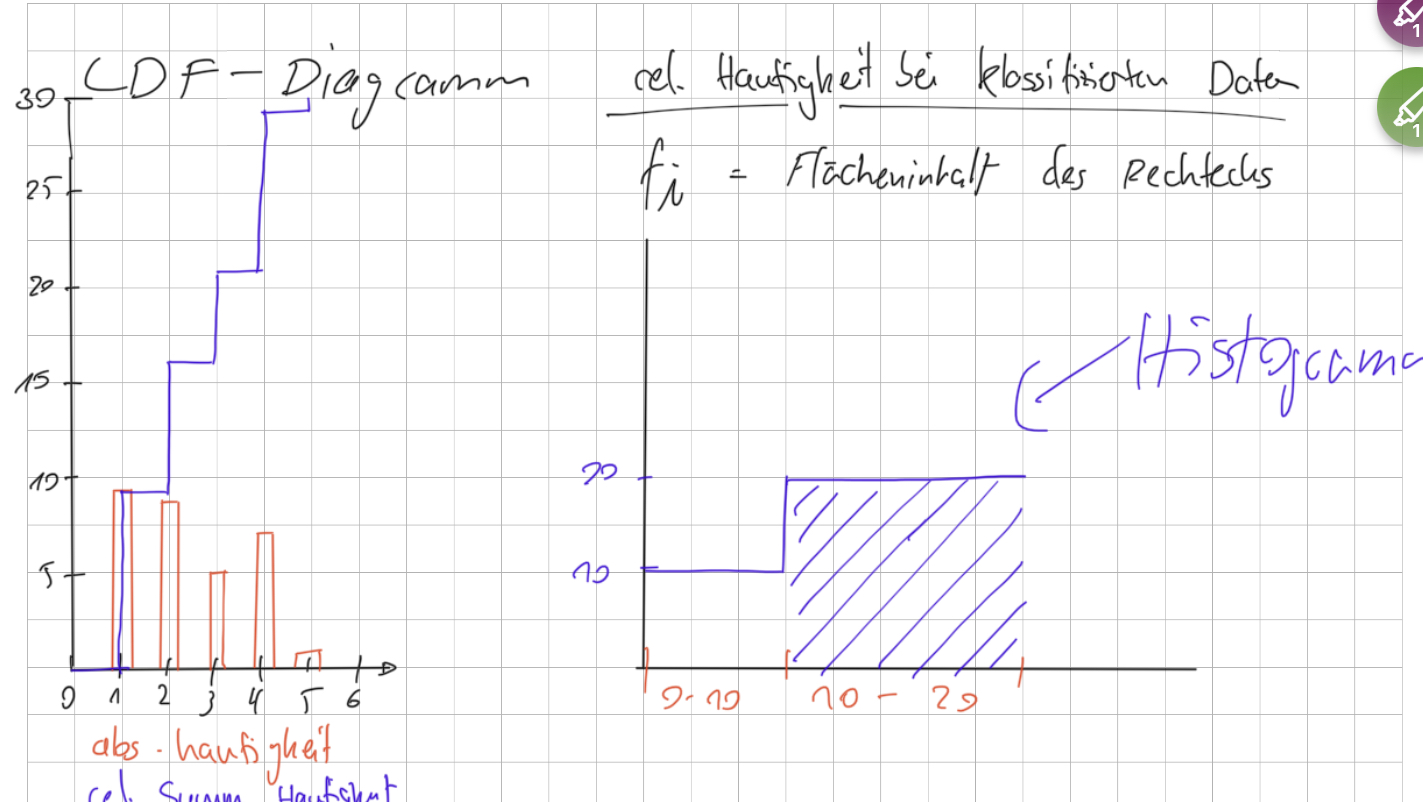
\includegraphics[height=6cm]{IMG_0205}


\section{Varianz}

\subsection{Arithmetisches Mittel}
Das Arithmetische Mittel wird auch als Durchschnitt bzwh. empirisches Mittel bezeichnet.

$
	\bar{x} = \sum_{i=1}^n a_i * f_i
$

\subsubsection{Bei klassierten Daten}

$
\bar{x} = \sum_{i=1}^n x_i
$
mit $ x_i $ als Klassenmitte

\subsection{Empirische Varianz / Stichprobenvarianz}
Beschreibt die mittlere quadratische Abweichung der einzelnen Werte vom empirischen Mittels.

	$
	\tilde{s}^2
	=
	\frac{1}{n} \cdot
	\sum_{i=1}^n (
	(a_i - \bar{x})^2* h_i)
	$
\\
alternativ

$
\tilde{s}^2 = \frac{1}{n} \cdot \sum_{i=1}^n (x_i - \bar{x})^2
$


\subsection{Standardabweichung}
 Die Standardabweichung ist ein Maß für die Streubreite der Werte eines Merkmals rund um dessen Mittelwert.
Vereinfacht gesagt, ist die Standardabweichung die durchschnittliche Entfernung aller gemessenen Ausprägungen eines Merkmals vom Durchschnitt.

$
\bar{s} = \sqrt{\tilde{s}^2}
$

\subsection{Korrigierte empirische Varianz}

$
\tilde{s}^2 = \frac{1}{n-1} \cdot \sum_{i=1}^n ((a_i - \bar{x})^2* h_i)
$

\subsection{Korrigierte Standardabweichung}

$
s = \sqrt{s^2}
$


\subfile{Boxplot.tex}

\end{document}


